\section{Analisis de la ordenacion por mezcla o mergesort}

En el ultimo ejercicio se ha analizado la eficiencia de uno de los algoritmos rapidos de ordenacion, en este caso el mergesort, que tiene una eficiencia teoríca de $O(n*log(n))$, a continuacion se muestra como en efecto la eficiencia del algoritmo implementado se ajusta a la funcion anterior:

%voy a poner mas datos rilax 
\begin{figure}[ht]
  \centering
  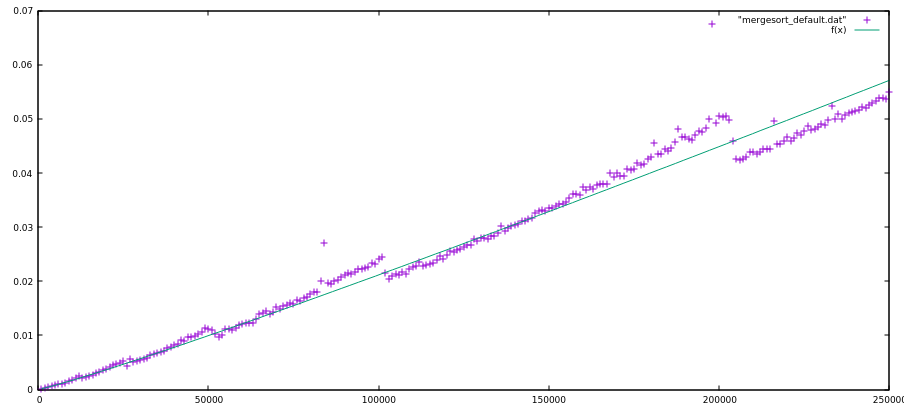
\includegraphics[width=0.5\textwidth]{./Imagenes/mergesort_fit.png}
  \caption{Grafica de la eficiencia del algoritmo mergesort}
\end{figure}

\subsection{Importancia del parametro UMBRAL\_MS}

A continuacion se muestra como afecta el parametro UMBRAL\_MS a la velocidad del algoritmo, ya que este indica el tamaño del caso base a partir del cual se realiza la ordenacion lineal y luego se combina la solucion.

\begin{figure}[H]
  \centering
  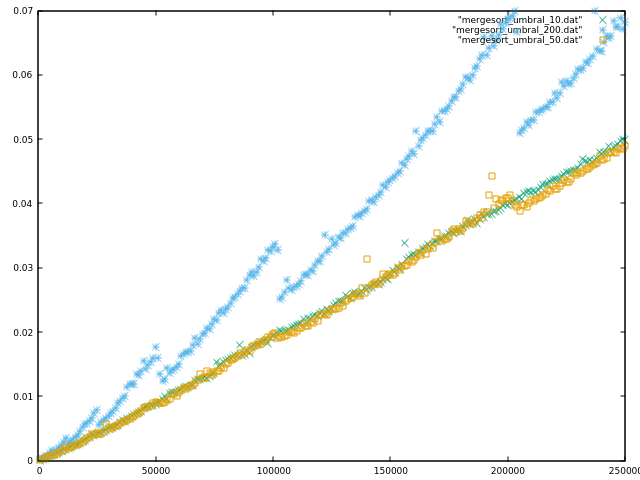
\includegraphics[width=0.5\textwidth]{./Imagenes/mergesort_umbral.png}
  \caption{Pruebas con diferentes umbrales del algoritmo mergesort}
\end{figure}
